\chapter{Industrial Context}
\label{chap:hexa}

\section{Introduction}

In order to understand the work that has been done during this PhD, it is preferable to first contextualize it. Hexaglobe will be presented first, along with their problems and motivations. Then, Section \ref{sec:hexadata} will introduce the internal datasets developed internally in order to approach the problems that we aim to solve. 

Hexaglobe provides all types of companies in the modern media landscape with technologies and professional services covering the entire process from video ingest to delivery.

Customers are numerous and diverse, from TV channels to radios and \ac{VOD} producers. Hexaglobe takes care of the whole video life cycle: uploading, storage, metadata extraction and management, encoding, referencing, search, and serving.

\section{Problems and motivations}

While classical software engineering is the right tool for encoding, managing, and serving the videos, it almost forces to consider them as impenetrable data blobs. Classical software engineering is very limited to the understanding and semantics that can be extracted from those data.

This is unfortunate. Being able to access the semantics of the videos would help improve the user experience in many ways \citep{contentretrieval}: it would make search more accurate, would allow for fine grain classification or help with recommendations. It would also be useful for the customers that would have more accurate insights into the type of videos that get more views, and would help data analytics with more intelligence. This is especially true for collaborative platforms, akin to YouTube, where the videos are uploaded by non professional people and the user given metadata cannot be relied on.

Very recent development have seen models such as \ac{CLIP} \citep{openaiclip} able to query images from natural languages, confirming the feasibility of the task.

The customer I have been affected to has a massive database of 9M+ user uploaded videos since 2006. That data has very little annotations and metadata, and it is fundamental that those videos can get recommended in a more impactful way, get more accurate categorization and more precise search. All in all, what is needed is to ease browsing and exploit that massive data and make sure nothing high value lies dormant or drowns in this data ocean.

It would also be interesting to modernize the older content with quality enhancement and super resolution techniques, a thing I kept in mind while learning about generative models. This, however, is far beyond the scope of this thesis.

\section{Data}
\label{sec:hexadata}

Throughout the thesis, three datasets have been created and are continuing to be developed as an ongoing process. Those datasets need to be refined, completed, and changed in order to fit the ever growing industrial needs. They are used for training and evaluating models before deployment.

Due to the confidential nature of the datasets, the nature of the data and example samples cannot be revealed.

\subsection{HActions}
\label{sec:hactions}

This first dataset has been manually labeled on my own. It contains pictures of natural images of people going on about what are supposed to be the 12 most popular activities on the website's videos, labeled A to M, plus an extra class that represents any other activity and another one for title screens / text screens showing no humans. The distribution of data samples is shown in Figure \ref{fig:xactions} and a few samples in Figure \ref{fig:xactionsamples}.

In many activity recognition tasks, the environment can be extremely informative. For instance, karting, canyoning, sailing, driving, climbing, all take place in different environments and there activity clues scattered all over the picture. However, our situation, those activities are decided by body position rather than environment. In some sense, sleeping, singing, dining, watching TV or playing games all take place in a domestic environment and a classifier would have very little clues in the environment to sort them out. Special care would be needed to make sure the classifier do not overfit on spurious background elements for instance.

Since training and inference on full videos would require a lot of compute, we instead assume that still pictures taken from the videos contain enough information for the classification task. 300 evenly spaced frames are extracted throughout videos that lasts more than one minute. That way the computation budget remains fixed and controlled. For comparison sake, if we were to use all the video frames with a temporality aware model, 300 frames would represent a video of 10s only. Even if a video aware model performed much better, the associated costs would be too high, and reducing the frame rate in training and inference would need another pass of video transcoding, which already is expensive.

Instead of randomly splitting the pictures among train / validation / test sets, we randomly split the \emph{videos} in those sets. Not doing this would create validation and test sets containing examples very similar to the ones in the train sets as nearby frames look similar. We aim to have a model that generalizes to videos outside the training set, not frames of a closed set of videos, thus the validation/test sets must contain frames of unseen videos.

\begin{figure}
    \centering
    \includegraphics[width=0.45\columnwidth]{20-files/train.pdf}
    \includegraphics[width=0.45\columnwidth]{20-files/test.pdf}
    \caption{Distribution of samples per classes in HActions.}
    \label{fig:xactions}
\end{figure}

\begin{figure}
    \centering
    \includegraphics[width=0.7\columnwidth]{20-files/actions.jpg}
    \caption{A few samples from HActions, with class label "none"}
    \label{fig:xactionsamples}
\end{figure}


\subsection{HFaces}

Automatic face recognition would bring very valuable metadata to our content. In our business, identifying celebrities in our domain is one of the core feature that the website's visitors would find valuable.

The dataset contains 8938 identities, but is growing every day as we wish to recognize more people. The distribution of the number of pictures per identities is shown in Figure \ref{fig:xfaces-num} and a few samples in Figure \ref{fig:xfaces-samples}. The dataset has been built with balance in mind. After collecting few very famous identities with web scraping, the labelers have been tasked to manually collect 100 pictures per identity when possible.

Our face dataset is divided into two data sources: faces coming from promotional pictures and coming from videos. Faces coming from pictures are easier to collect but are prone to domain mismatch with videos as they are cleaner: the faces are usually not occluded, there is no motion blur, lighting is good and people tend to smile. In videos, none of this might hold true. We collected many pictures from photos and a smaller bunch from videos in order to evaluate and eventually mitigate the domain mismatch between both.

\begin{figure}
    \centering
    \includegraphics[width=0.7\columnwidth]{20-files/xfaces-num.pdf}
    \caption{Number of examples per identities in the photos subset of HFaces (sorted). Most identities have between 10 and 100 samples.}
    \label{fig:xfaces-num}
\end{figure}

\begin{figure}
    \centering
    \includegraphics[scale=1.5]{20-files/xfaces-samples.jpg}
    \caption{Samples from HFaces. Top row: extracted from pictures. Bottom row: extracted from videos.}
    \label{fig:xfaces-samples}
\end{figure}

The dataset has been complemented with MS1Mv2 \citep{celeb1m} to provide the so-called "distractors", developped in section \ref{sec:our-facerec}.

\subsection{HHistory}
\label{sec:hhistory}
\begin{figure}
    \centering
    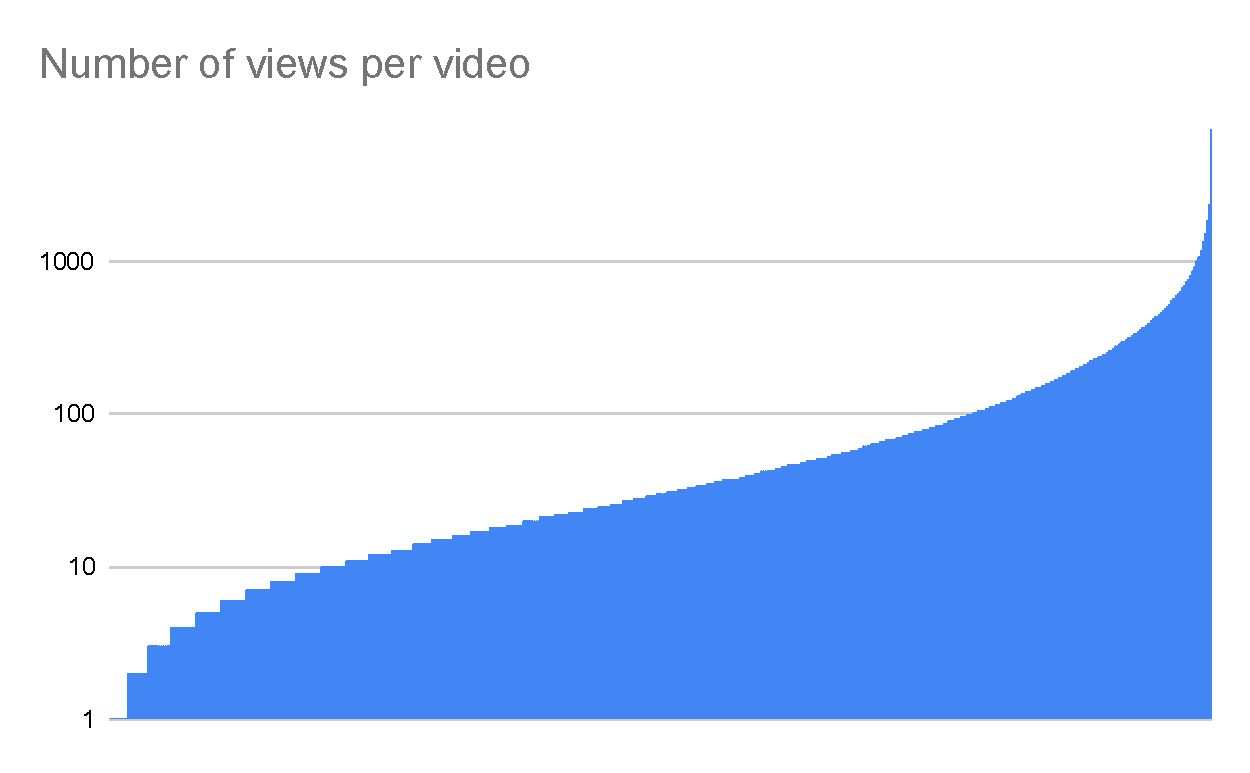
\includegraphics[width=\columnwidth]{20-files/video_views.pdf}
    \caption{Number of views per videos (sorted). Each video is a thin vertical bar.}
    \label{fig:xhistory-views}
\end{figure}

Finally, there is a dataset of premium users' browsing history. This dataset is here to provide historical data for building a recommender system, analyze trends, study semantic proximity of items, etc. This could be useful in various way : videos frequently watched together can serve as contrastive / metric learning dataset to learn about visual features that makes them similar, can learn about tag proximity as well, etc. This dataset can be of many uses and the only metric really lacking is the lenght of watch time per video in order to assess the interest of the user.

Premium content is only a subset of the whole content. The dataset has 135,984 users (content uploader), 3,673 channels and 139,711 videos. The distribution of views is in Figure \ref{fig:xhistory-views}. It contains various user information, many being optional:

\begin{enumerate}
    \item user ID
    \item username
    \item country / region
    \item gender
    \item liked videos (and the like action timestamp)
    \item disliked videos (and the dislike action timestamp)
    \item favorited videos
    \item watched videos (and their watch timestamp)
    \item channels subscriptions
\end{enumerate}

Similarly, metadata about videos are:

\begin{enumerate}
    \item video ID
    \item main category
    \item the uploader's channel ID
    \item people appearing in the video (from the face recognition model or the previous system)
    \item title (possibly in multiple languages)
    \item various free form tags chosen by the uploader
    \item video encoding quality
    \item upload timestamp
\end{enumerate}

Finally, each channel has popularity scores per category and region.

\subsection{A note about open datasets}

The reader used to academic benchmark and comparisons might object and argue that there are open datasets covering the kind of problems dealt with here. Indeed none of those tasks are new. That being said, each use case is unique in its own way and models fitted on those datasets can't be straightly used for the industrial needs.

HActivity can be thought to be similar to YouTube-8M \citep{youtube8m}. The actions in HActivity have zero overlap with YouTube-8M, so it definitely cannot be used there. Also, as discussed before, the actions in YouTube-8M are often highly informed by environmental clues and much less by body pose.

HFaces resembles CelebA \citep{celeba} / MS1M \citep{celeb1m}. Both those datasets have a vast majority of neutral faces facing the camera. In our situation, the face are quite often non neutral and highly expressive, like faces during sports could be, are quite often not facing the camera, suffer from motion blur, occlusions, and MPEG encoding artifacts.

HHistory is harder to relate to MovieLens \citep{movielens} and Netflix \citep{netflix}. Those datasets are centered around ratings. While HHistory has some, they are both binary and scarce, and most of the training supervision has to be extracted from watch history instead.

\section{Machines}

To work, Hexaglobe provides me three machines, hosted by our Cloud computing provider.

\begin{enumerate}
    \item gpu1 has 2 NVIDIA GTX 1080 Ti and is used mainly for production and inference.
    \item gpu2 has 4 NVIDIA RTX 2080 and is used for my main experiments. It allows me to iterate quickly during development by using large batch sizes.
    \item gpu3 has 2 NVIDIA RTX 2080. This machine is used for runs that I don't mind waiting or for side experiments.
\end{enumerate}

The university also provided several clusters that I could use when working on public datasets.

\section{Conclusion}
%FIXME
In this chapter, we presented the company who supported the thesis and their industrial needs: they provide video platforms to customers. In order to improve their products, they would like to explore what Deep Learning has to offer for extracting metadata. Those metadata would be used to enrich searchability, sorting, user experience and recommendation. It then appears coherent to first focus on extracting activity and face recognition to collect the most important features, then build a recommender system using them.

We are developing three datasets, one for each task: HActivity for activity recognition, HFaces for face recognition, and HHistory for the recommender system.

In the next chapters, we will be exploiting those datasets in order to develop and improve models.